%\documentclass{standalone}
%\usepackage{tikz}
%\usetikzlibrary{patterns,plotmarks}
%\begin{document}
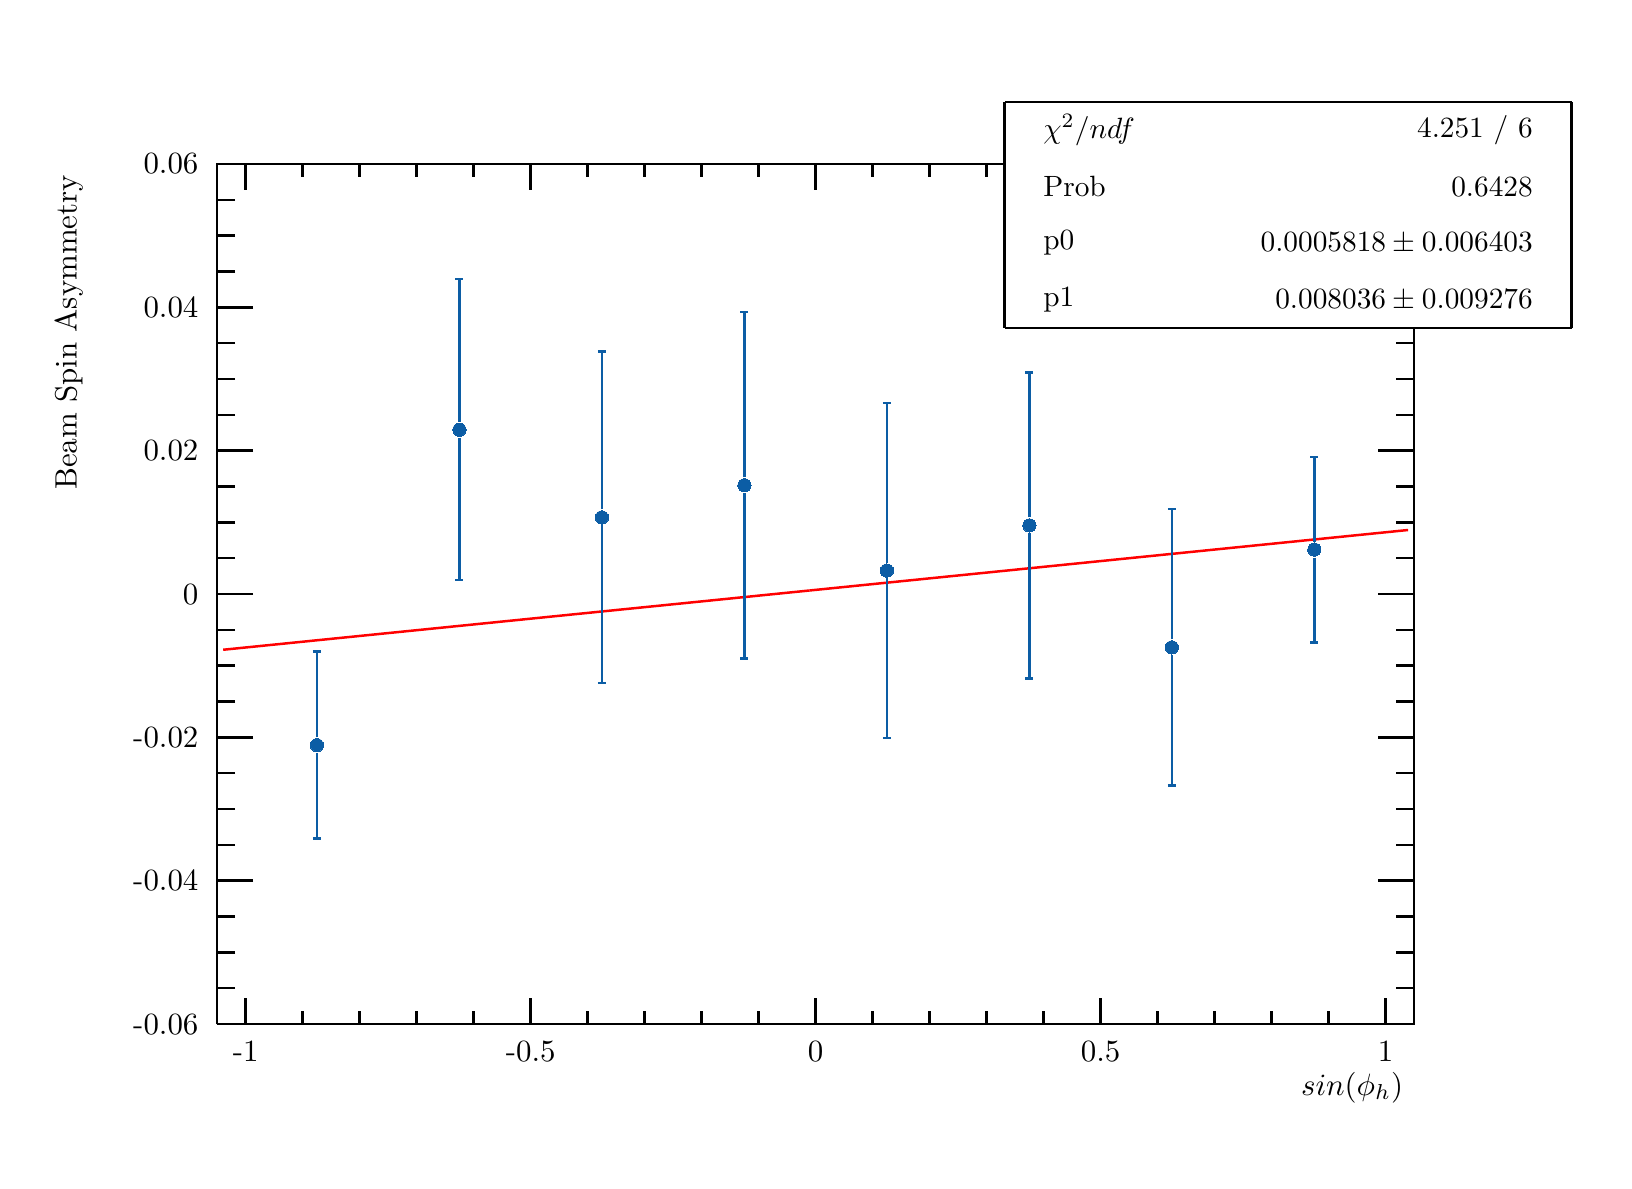
\begin{tikzpicture}
\def\CheckTikzLibraryLoaded#1{ \ifcsname tikz@library@#1@loaded\endcsname \else \PackageWarning{tikz}{usetikzlibrary{#1} is missing in the preamble.} \fi }
\CheckTikzLibraryLoaded{patterns}
\CheckTikzLibraryLoaded{plotmarks}
\pgfdeclareplotmark{cross} {
\pgfpathmoveto{\pgfpoint{-0.3\pgfplotmarksize}{\pgfplotmarksize}}
\pgfpathlineto{\pgfpoint{+0.3\pgfplotmarksize}{\pgfplotmarksize}}
\pgfpathlineto{\pgfpoint{+0.3\pgfplotmarksize}{0.3\pgfplotmarksize}}
\pgfpathlineto{\pgfpoint{+1\pgfplotmarksize}{0.3\pgfplotmarksize}}
\pgfpathlineto{\pgfpoint{+1\pgfplotmarksize}{-0.3\pgfplotmarksize}}
\pgfpathlineto{\pgfpoint{+0.3\pgfplotmarksize}{-0.3\pgfplotmarksize}}
\pgfpathlineto{\pgfpoint{+0.3\pgfplotmarksize}{-1.\pgfplotmarksize}}
\pgfpathlineto{\pgfpoint{-0.3\pgfplotmarksize}{-1.\pgfplotmarksize}}
\pgfpathlineto{\pgfpoint{-0.3\pgfplotmarksize}{-0.3\pgfplotmarksize}}
\pgfpathlineto{\pgfpoint{-1.\pgfplotmarksize}{-0.3\pgfplotmarksize}}
\pgfpathlineto{\pgfpoint{-1.\pgfplotmarksize}{0.3\pgfplotmarksize}}
\pgfpathlineto{\pgfpoint{-0.3\pgfplotmarksize}{0.3\pgfplotmarksize}}
\pgfpathclose
\pgfusepathqstroke
}
\pgfdeclareplotmark{cross*} {
\pgfpathmoveto{\pgfpoint{-0.3\pgfplotmarksize}{\pgfplotmarksize}}
\pgfpathlineto{\pgfpoint{+0.3\pgfplotmarksize}{\pgfplotmarksize}}
\pgfpathlineto{\pgfpoint{+0.3\pgfplotmarksize}{0.3\pgfplotmarksize}}
\pgfpathlineto{\pgfpoint{+1\pgfplotmarksize}{0.3\pgfplotmarksize}}
\pgfpathlineto{\pgfpoint{+1\pgfplotmarksize}{-0.3\pgfplotmarksize}}
\pgfpathlineto{\pgfpoint{+0.3\pgfplotmarksize}{-0.3\pgfplotmarksize}}
\pgfpathlineto{\pgfpoint{+0.3\pgfplotmarksize}{-1.\pgfplotmarksize}}
\pgfpathlineto{\pgfpoint{-0.3\pgfplotmarksize}{-1.\pgfplotmarksize}}
\pgfpathlineto{\pgfpoint{-0.3\pgfplotmarksize}{-0.3\pgfplotmarksize}}
\pgfpathlineto{\pgfpoint{-1.\pgfplotmarksize}{-0.3\pgfplotmarksize}}
\pgfpathlineto{\pgfpoint{-1.\pgfplotmarksize}{0.3\pgfplotmarksize}}
\pgfpathlineto{\pgfpoint{-0.3\pgfplotmarksize}{0.3\pgfplotmarksize}}
\pgfpathclose
\pgfusepathqfillstroke
}
\pgfdeclareplotmark{newstar} {
\pgfpathmoveto{\pgfqpoint{0pt}{\pgfplotmarksize}}
\pgfpathlineto{\pgfqpointpolar{44}{0.5\pgfplotmarksize}}
\pgfpathlineto{\pgfqpointpolar{18}{\pgfplotmarksize}}
\pgfpathlineto{\pgfqpointpolar{-20}{0.5\pgfplotmarksize}}
\pgfpathlineto{\pgfqpointpolar{-54}{\pgfplotmarksize}}
\pgfpathlineto{\pgfqpointpolar{-90}{0.5\pgfplotmarksize}}
\pgfpathlineto{\pgfqpointpolar{234}{\pgfplotmarksize}}
\pgfpathlineto{\pgfqpointpolar{198}{0.5\pgfplotmarksize}}
\pgfpathlineto{\pgfqpointpolar{162}{\pgfplotmarksize}}
\pgfpathlineto{\pgfqpointpolar{134}{0.5\pgfplotmarksize}}
\pgfpathclose
\pgfusepathqstroke
}
\pgfdeclareplotmark{newstar*} {
\pgfpathmoveto{\pgfqpoint{0pt}{\pgfplotmarksize}}
\pgfpathlineto{\pgfqpointpolar{44}{0.5\pgfplotmarksize}}
\pgfpathlineto{\pgfqpointpolar{18}{\pgfplotmarksize}}
\pgfpathlineto{\pgfqpointpolar{-20}{0.5\pgfplotmarksize}}
\pgfpathlineto{\pgfqpointpolar{-54}{\pgfplotmarksize}}
\pgfpathlineto{\pgfqpointpolar{-90}{0.5\pgfplotmarksize}}
\pgfpathlineto{\pgfqpointpolar{234}{\pgfplotmarksize}}
\pgfpathlineto{\pgfqpointpolar{198}{0.5\pgfplotmarksize}}
\pgfpathlineto{\pgfqpointpolar{162}{\pgfplotmarksize}}
\pgfpathlineto{\pgfqpointpolar{134}{0.5\pgfplotmarksize}}
\pgfpathclose
\pgfusepathqfillstroke
}
\definecolor{c}{rgb}{1,1,1};
\draw [color=c, fill=c] (0,0) rectangle (20,14.3719);
\draw [color=c, fill=c] (2.4,1.72462) rectangle (17.6,12.6472);
\definecolor{c}{rgb}{0,0,0};
\draw [c,line width=0.9] (2.4,1.72462) -- (2.4,12.6472) -- (17.6,12.6472) -- (17.6,1.72462) -- (2.4,1.72462);
\definecolor{c}{rgb}{1,1,1};
\draw [color=c, fill=c] (2.4,1.72462) rectangle (17.6,12.6472);
\definecolor{c}{rgb}{0,0,0};
\draw [c,line width=0.9] (2.4,1.72462) -- (2.4,12.6472) -- (17.6,12.6472) -- (17.6,1.72462) -- (2.4,1.72462);
\draw [c,line width=0.9] (2.4,1.72462) -- (17.6,1.72462);
\draw [c,line width=0.9] (2.7619,2.0523) -- (2.7619,1.72462);
\draw [c,line width=0.9] (3.48571,1.88846) -- (3.48571,1.72462);
\draw [c,line width=0.9] (4.20952,1.88846) -- (4.20952,1.72462);
\draw [c,line width=0.9] (4.93333,1.88846) -- (4.93333,1.72462);
\draw [c,line width=0.9] (5.65714,1.88846) -- (5.65714,1.72462);
\draw [c,line width=0.9] (6.38095,2.0523) -- (6.38095,1.72462);
\draw [c,line width=0.9] (7.10476,1.88846) -- (7.10476,1.72462);
\draw [c,line width=0.9] (7.82857,1.88846) -- (7.82857,1.72462);
\draw [c,line width=0.9] (8.55238,1.88846) -- (8.55238,1.72462);
\draw [c,line width=0.9] (9.27619,1.88846) -- (9.27619,1.72462);
\draw [c,line width=0.9] (10,2.0523) -- (10,1.72462);
\draw [c,line width=0.9] (10.7238,1.88846) -- (10.7238,1.72462);
\draw [c,line width=0.9] (11.4476,1.88846) -- (11.4476,1.72462);
\draw [c,line width=0.9] (12.1714,1.88846) -- (12.1714,1.72462);
\draw [c,line width=0.9] (12.8952,1.88846) -- (12.8952,1.72462);
\draw [c,line width=0.9] (13.619,2.0523) -- (13.619,1.72462);
\draw [c,line width=0.9] (14.3429,1.88846) -- (14.3429,1.72462);
\draw [c,line width=0.9] (15.0667,1.88846) -- (15.0667,1.72462);
\draw [c,line width=0.9] (15.7905,1.88846) -- (15.7905,1.72462);
\draw [c,line width=0.9] (16.5143,1.88846) -- (16.5143,1.72462);
\draw [c,line width=0.9] (17.2381,2.0523) -- (17.2381,1.72462);
\draw [c,line width=0.9] (2.7619,2.0523) -- (2.7619,1.72462);
\draw [c,line width=0.9] (17.2381,2.0523) -- (17.2381,1.72462);
\draw [anchor=base] (2.7619,1.25035) node[scale=1.11607, color=c, rotate=0]{-1};
\draw [anchor=base] (6.38095,1.25035) node[scale=1.11607, color=c, rotate=0]{-0.5};
\draw [anchor=base] (10,1.25035) node[scale=1.11607, color=c, rotate=0]{0};
\draw [anchor=base] (13.619,1.25035) node[scale=1.11607, color=c, rotate=0]{0.5};
\draw [anchor=base] (17.2381,1.25035) node[scale=1.11607, color=c, rotate=0]{1};
\draw [anchor= east] (17.6,0.919799) node[scale=1.11607, color=c, rotate=0]{$sin(\phi_{h})$};
\draw [c,line width=0.9] (2.4,12.6472) -- (17.6,12.6472);
\draw [c,line width=0.9] (2.7619,12.3196) -- (2.7619,12.6472);
\draw [c,line width=0.9] (3.48571,12.4834) -- (3.48571,12.6472);
\draw [c,line width=0.9] (4.20952,12.4834) -- (4.20952,12.6472);
\draw [c,line width=0.9] (4.93333,12.4834) -- (4.93333,12.6472);
\draw [c,line width=0.9] (5.65714,12.4834) -- (5.65714,12.6472);
\draw [c,line width=0.9] (6.38095,12.3196) -- (6.38095,12.6472);
\draw [c,line width=0.9] (7.10476,12.4834) -- (7.10476,12.6472);
\draw [c,line width=0.9] (7.82857,12.4834) -- (7.82857,12.6472);
\draw [c,line width=0.9] (8.55238,12.4834) -- (8.55238,12.6472);
\draw [c,line width=0.9] (9.27619,12.4834) -- (9.27619,12.6472);
\draw [c,line width=0.9] (10,12.3196) -- (10,12.6472);
\draw [c,line width=0.9] (10.7238,12.4834) -- (10.7238,12.6472);
\draw [c,line width=0.9] (11.4476,12.4834) -- (11.4476,12.6472);
\draw [c,line width=0.9] (12.1714,12.4834) -- (12.1714,12.6472);
\draw [c,line width=0.9] (12.8952,12.4834) -- (12.8952,12.6472);
\draw [c,line width=0.9] (13.619,12.3196) -- (13.619,12.6472);
\draw [c,line width=0.9] (14.3429,12.4834) -- (14.3429,12.6472);
\draw [c,line width=0.9] (15.0667,12.4834) -- (15.0667,12.6472);
\draw [c,line width=0.9] (15.7905,12.4834) -- (15.7905,12.6472);
\draw [c,line width=0.9] (16.5143,12.4834) -- (16.5143,12.6472);
\draw [c,line width=0.9] (17.2381,12.3196) -- (17.2381,12.6472);
\draw [c,line width=0.9] (2.7619,12.3196) -- (2.7619,12.6472);
\draw [c,line width=0.9] (17.2381,12.3196) -- (17.2381,12.6472);
\draw [c,line width=0.9] (2.4,1.72462) -- (2.4,12.6472);
\draw [c,line width=0.9] (2.856,1.72462) -- (2.4,1.72462);
\draw [c,line width=0.9] (2.628,2.17973) -- (2.4,2.17973);
\draw [c,line width=0.9] (2.628,2.63484) -- (2.4,2.63484);
\draw [c,line width=0.9] (2.628,3.08995) -- (2.4,3.08995);
\draw [c,line width=0.9] (2.856,3.54506) -- (2.4,3.54506);
\draw [c,line width=0.9] (2.628,4.00017) -- (2.4,4.00017);
\draw [c,line width=0.9] (2.628,4.45528) -- (2.4,4.45528);
\draw [c,line width=0.9] (2.628,4.91039) -- (2.4,4.91039);
\draw [c,line width=0.9] (2.856,5.36549) -- (2.4,5.36549);
\draw [c,line width=0.9] (2.628,5.8206) -- (2.4,5.8206);
\draw [c,line width=0.9] (2.628,6.27571) -- (2.4,6.27571);
\draw [c,line width=0.9] (2.628,6.73082) -- (2.4,6.73082);
\draw [c,line width=0.9] (2.856,7.18593) -- (2.4,7.18593);
\draw [c,line width=0.9] (2.628,7.64104) -- (2.4,7.64104);
\draw [c,line width=0.9] (2.628,8.09615) -- (2.4,8.09615);
\draw [c,line width=0.9] (2.628,8.55126) -- (2.4,8.55126);
\draw [c,line width=0.9] (2.856,9.00637) -- (2.4,9.00637);
\draw [c,line width=0.9] (2.628,9.46147) -- (2.4,9.46147);
\draw [c,line width=0.9] (2.628,9.91658) -- (2.4,9.91658);
\draw [c,line width=0.9] (2.628,10.3717) -- (2.4,10.3717);
\draw [c,line width=0.9] (2.856,10.8268) -- (2.4,10.8268);
\draw [c,line width=0.9] (2.628,11.2819) -- (2.4,11.2819);
\draw [c,line width=0.9] (2.628,11.737) -- (2.4,11.737);
\draw [c,line width=0.9] (2.628,12.1921) -- (2.4,12.1921);
\draw [c,line width=0.9] (2.856,12.6472) -- (2.4,12.6472);
\draw [anchor= east] (2.3,1.72462) node[scale=1.11607, color=c, rotate=0]{-0.06};
\draw [anchor= east] (2.3,3.54506) node[scale=1.11607, color=c, rotate=0]{-0.04};
\draw [anchor= east] (2.3,5.36549) node[scale=1.11607, color=c, rotate=0]{-0.02};
\draw [anchor= east] (2.3,7.18593) node[scale=1.11607, color=c, rotate=0]{0};
\draw [anchor= east] (2.3,9.00637) node[scale=1.11607, color=c, rotate=0]{0.02};
\draw [anchor= east] (2.3,10.8268) node[scale=1.11607, color=c, rotate=0]{0.04};
\draw [anchor= east] (2.3,12.6472) node[scale=1.11607, color=c, rotate=0]{0.06};
\draw [anchor= east] (0.519095,12.6472) node[scale=1.11607, color=c, rotate=90]{Beam Spin Asymmetry};
\draw [c,line width=0.9] (17.6,1.72462) -- (17.6,12.6472);
\draw [c,line width=0.9] (17.144,1.72462) -- (17.6,1.72462);
\draw [c,line width=0.9] (17.372,2.17973) -- (17.6,2.17973);
\draw [c,line width=0.9] (17.372,2.63484) -- (17.6,2.63484);
\draw [c,line width=0.9] (17.372,3.08995) -- (17.6,3.08995);
\draw [c,line width=0.9] (17.144,3.54506) -- (17.6,3.54506);
\draw [c,line width=0.9] (17.372,4.00017) -- (17.6,4.00017);
\draw [c,line width=0.9] (17.372,4.45528) -- (17.6,4.45528);
\draw [c,line width=0.9] (17.372,4.91039) -- (17.6,4.91039);
\draw [c,line width=0.9] (17.144,5.36549) -- (17.6,5.36549);
\draw [c,line width=0.9] (17.372,5.8206) -- (17.6,5.8206);
\draw [c,line width=0.9] (17.372,6.27571) -- (17.6,6.27571);
\draw [c,line width=0.9] (17.372,6.73082) -- (17.6,6.73082);
\draw [c,line width=0.9] (17.144,7.18593) -- (17.6,7.18593);
\draw [c,line width=0.9] (17.372,7.64104) -- (17.6,7.64104);
\draw [c,line width=0.9] (17.372,8.09615) -- (17.6,8.09615);
\draw [c,line width=0.9] (17.372,8.55126) -- (17.6,8.55126);
\draw [c,line width=0.9] (17.144,9.00637) -- (17.6,9.00637);
\draw [c,line width=0.9] (17.372,9.46147) -- (17.6,9.46147);
\draw [c,line width=0.9] (17.372,9.91658) -- (17.6,9.91658);
\draw [c,line width=0.9] (17.372,10.3717) -- (17.6,10.3717);
\draw [c,line width=0.9] (17.144,10.8268) -- (17.6,10.8268);
\draw [c,line width=0.9] (17.372,11.2819) -- (17.6,11.2819);
\draw [c,line width=0.9] (17.372,11.737) -- (17.6,11.737);
\draw [c,line width=0.9] (17.372,12.1921) -- (17.6,12.1921);
\draw [c,line width=0.9] (17.144,12.6472) -- (17.6,12.6472);
\definecolor{c}{rgb}{0.0470588,0.364706,0.647059};
\foreach \P in {(3.66667,5.26642), (5.47619,9.27285), (7.28571,8.15942), (9.09524,8.56666), (10.9048,7.48404), (12.7143,8.05755), (14.5238,6.50868), (16.3333,7.75052)}{\draw[mark options={color=c,fill=c},mark size=2.402402pt, line width=0.000000pt,
 mark=*] plot coordinates {\P};}
\definecolor{c}{rgb}{1,0,0};
\draw [c,line width=0.9] (2.476,6.47851) -- (2.628,6.49387) -- (2.78,6.50923) -- (2.932,6.52459) -- (3.084,6.53995) -- (3.236,6.55531) -- (3.388,6.57067) -- (3.54,6.58603) -- (3.692,6.6014) -- (3.844,6.61676) -- (3.996,6.63212) -- (4.148,6.64748) --
 (4.3,6.66284) -- (4.452,6.6782) -- (4.604,6.69356) -- (4.756,6.70892) -- (4.908,6.72429) -- (5.06,6.73965) -- (5.212,6.75501) -- (5.364,6.77037) -- (5.516,6.78573) -- (5.668,6.80109) -- (5.82,6.81645) -- (5.972,6.83181) -- (6.124,6.84717) --
 (6.276,6.86253) -- (6.428,6.8779) -- (6.58,6.89326) -- (6.732,6.90862) -- (6.884,6.92398) -- (7.036,6.93934) -- (7.188,6.9547) -- (7.34,6.97006) -- (7.492,6.98542) -- (7.644,7.00079) -- (7.796,7.01615) -- (7.948,7.03151) -- (8.1,7.04687) --
 (8.252,7.06223) -- (8.404,7.07759) -- (8.556,7.09295) -- (8.708,7.10831) -- (8.86,7.12367) -- (9.012,7.13904) -- (9.164,7.1544) -- (9.316,7.16976) -- (9.468,7.18512) -- (9.62,7.20048) -- (9.772,7.21584) -- (9.924,7.2312);
\draw [c,line width=0.9] (9.924,7.2312) -- (10.076,7.24656) -- (10.228,7.26192) -- (10.38,7.27729) -- (10.532,7.29265) -- (10.684,7.30801) -- (10.836,7.32337) -- (10.988,7.33873) -- (11.14,7.35409) -- (11.292,7.36945) -- (11.444,7.38481) --
 (11.596,7.40017) -- (11.748,7.41554) -- (11.9,7.4309) -- (12.052,7.44626) -- (12.204,7.46162) -- (12.356,7.47698) -- (12.508,7.49234) -- (12.66,7.5077) -- (12.812,7.52306) -- (12.964,7.53842) -- (13.116,7.55379) -- (13.268,7.56915) --
 (13.42,7.58451) -- (13.572,7.59987) -- (13.724,7.61523) -- (13.876,7.63059) -- (14.028,7.64595) -- (14.18,7.66131) -- (14.332,7.67667) -- (14.484,7.69204) -- (14.636,7.7074) -- (14.788,7.72276) -- (14.94,7.73812) -- (15.092,7.75348) --
 (15.244,7.76884) -- (15.396,7.7842) -- (15.548,7.79956) -- (15.7,7.81493) -- (15.852,7.83029) -- (16.004,7.84565) -- (16.156,7.86101) -- (16.308,7.87637) -- (16.46,7.89173) -- (16.612,7.90709) -- (16.764,7.92245) -- (16.916,7.93781) --
 (17.068,7.95318) -- (17.22,7.96854) -- (17.372,7.9839);
\draw [c,line width=0.9] (17.372,7.9839) -- (17.524,7.99926);
\definecolor{c}{rgb}{1,1,1};
\draw [color=c, fill=c] (12.4,10.5633) rectangle (19.6,13.4377);
\definecolor{c}{rgb}{0,0,0};
\draw [c,line width=0.9] (12.4,10.5633) -- (19.6,10.5633);
\draw [c,line width=0.9] (19.6,10.5633) -- (19.6,13.4377);
\draw [c,line width=0.9] (19.6,13.4377) -- (12.4,13.4377);
\draw [c,line width=0.9] (12.4,13.4377) -- (12.4,10.5633);
\draw [anchor= west] (12.76,13.0784) node[scale=1.06026, color=c, rotate=0]{$\chi^{2} / ndf $};
\draw [anchor= east] (19.24,13.0784) node[scale=1.06026, color=c, rotate=0]{ 4.251 / 6};
\draw [anchor= west] (12.76,12.3598) node[scale=1.06026, color=c, rotate=0]{Prob  };
\draw [anchor= east] (19.24,12.3598) node[scale=1.06026, color=c, rotate=0]{ 0.6428};
\draw [anchor= west] (12.76,11.6412) node[scale=1.06026, color=c, rotate=0]{p0       };
\draw [anchor= east] (19.24,11.6412) node[scale=1.06026, color=c, rotate=0]{$ 0.0005818 \pm 0.006403$};
\draw [anchor= west] (12.76,10.9226) node[scale=1.06026, color=c, rotate=0]{p1       };
\draw [anchor= east] (19.24,10.9226) node[scale=1.06026, color=c, rotate=0]{$ 0.008036 \pm 0.009276$};
\definecolor{c}{rgb}{0.0470588,0.364706,0.647059};
\draw [c,line width=0.9] (3.66667,5.36693) -- (3.66667,6.45344);
\draw [c,line width=0.9] (3.66667,5.16592) -- (3.66667,4.07941);
\draw [c,line width=0.9] (3.61642,6.45344) -- (3.71692,6.45344);
\draw [c,line width=0.9] (3.61642,4.07941) -- (3.71692,4.07941);
\draw [c,line width=0.9] (5.47619,9.37335) -- (5.47619,11.1841);
\draw [c,line width=0.9] (5.47619,9.17235) -- (5.47619,7.36157);
\draw [c,line width=0.9] (5.42594,11.1841) -- (5.52644,11.1841);
\draw [c,line width=0.9] (5.42594,7.36157) -- (5.52644,7.36157);
\draw [c,line width=0.9] (7.28571,8.25993) -- (7.28571,10.2643);
\draw [c,line width=0.9] (7.28571,8.05892) -- (7.28571,6.05456);
\draw [c,line width=0.9] (7.23546,10.2643) -- (7.33597,10.2643);
\draw [c,line width=0.9] (7.23546,6.05456) -- (7.33597,6.05456);
\draw [c,line width=0.9] (9.09524,8.66716) -- (9.09524,10.7652);
\draw [c,line width=0.9] (9.09524,8.46615) -- (9.09524,6.36809);
\draw [c,line width=0.9] (9.04499,10.7652) -- (9.14549,10.7652);
\draw [c,line width=0.9] (9.04499,6.36809) -- (9.14549,6.36809);
\draw [c,line width=0.9] (10.9048,7.58454) -- (10.9048,9.61062);
\draw [c,line width=0.9] (10.9048,7.38353) -- (10.9048,5.35745);
\draw [c,line width=0.9] (10.8545,9.61062) -- (10.955,9.61062);
\draw [c,line width=0.9] (10.8545,5.35745) -- (10.955,5.35745);
\draw [c,line width=0.9] (12.7143,8.15805) -- (12.7143,10.0012);
\draw [c,line width=0.9] (12.7143,7.95704) -- (12.7143,6.11386);
\draw [c,line width=0.9] (12.664,10.0012) -- (12.7645,10.0012);
\draw [c,line width=0.9] (12.664,6.11386) -- (12.7645,6.11386);
\draw [c,line width=0.9] (14.5238,6.60919) -- (14.5238,8.26431);
\draw [c,line width=0.9] (14.5238,6.40818) -- (14.5238,4.75306);
\draw [c,line width=0.9] (14.4736,8.26431) -- (14.5741,8.26431);
\draw [c,line width=0.9] (14.4736,4.75306) -- (14.5741,4.75306);
\draw [c,line width=0.9] (16.3333,7.85103) -- (16.3333,8.92905);
\draw [c,line width=0.9] (16.3333,7.65002) -- (16.3333,6.572);
\draw [c,line width=0.9] (16.2831,8.92905) -- (16.3836,8.92905);
\draw [c,line width=0.9] (16.2831,6.572) -- (16.3836,6.572);
\definecolor{c}{rgb}{1,1,1};
\draw [color=c, fill=c] (12.4,10.5633) rectangle (19.6,13.4377);
\definecolor{c}{rgb}{0,0,0};
\draw [c,line width=0.9] (12.4,10.5633) -- (19.6,10.5633);
\draw [c,line width=0.9] (19.6,10.5633) -- (19.6,13.4377);
\draw [c,line width=0.9] (19.6,13.4377) -- (12.4,13.4377);
\draw [c,line width=0.9] (12.4,13.4377) -- (12.4,10.5633);
\draw [anchor= west] (12.76,13.0784) node[scale=1.06026, color=c, rotate=0]{$\chi^{2} / ndf $};
\draw [anchor= east] (19.24,13.0784) node[scale=1.06026, color=c, rotate=0]{ 4.251 / 6};
\draw [anchor= west] (12.76,12.3598) node[scale=1.06026, color=c, rotate=0]{Prob  };
\draw [anchor= east] (19.24,12.3598) node[scale=1.06026, color=c, rotate=0]{ 0.6428};
\draw [anchor= west] (12.76,11.6412) node[scale=1.06026, color=c, rotate=0]{p0       };
\draw [anchor= east] (19.24,11.6412) node[scale=1.06026, color=c, rotate=0]{$ 0.0005818 \pm 0.006403$};
\draw [anchor= west] (12.76,10.9226) node[scale=1.06026, color=c, rotate=0]{p1       };
\draw [anchor= east] (19.24,10.9226) node[scale=1.06026, color=c, rotate=0]{$ 0.008036 \pm 0.009276$};
\end{tikzpicture}
%\end{document}
